\documentclass[11pt]{article}

\usepackage[english]{babel}
\usepackage[utf8]{inputenc}
\usepackage{amsmath}
\usepackage{amssymb}
\usepackage{graphicx}
\usepackage[colorinlistoftodos]{todonotes}
\usepackage{listings,multicol}
\usepackage{textcomp}
\usepackage{hyperref}
\usepackage{longtable}

\setlength{\oddsidemargin}{0.5cm} \setlength{\evensidemargin}{0cm}
\setlength{\textwidth}{16cm} \setlength{\textheight}{23cm}
\setlength{\topmargin}{-0.5cm}
\textheight 21.5cm


\begin{document}

\title{L3 NUMERICO UCSC}

\begin{minipage}{0.15\textwidth}

\includegraphics[width=\textwidth]{ucsc.png}
\end{minipage}
\begin{minipage}{0.9\textwidth}
{UNIVERSIDAD CAT\'OLICA}\\ 
{DE LA SANT\'ISIMA CONCEPCI\'ON}\\
{DEPARTAMENTO DE MATEM\'ATICA}\\ 
{ Y F\'ISICA APLICADAS}\\
\rule{0.66\textwidth}{.5pt} %Franco A. Milanese
\end{minipage}

\vspace*{0.5cm} \centerline {\bf\underline{Laboratorio 3, C\'alculo Num\'erico  IN1012C }}
\centerline{\textrm{Semana 6 de abril de 2015}}  \vspace{0.2cm}


% \textbf{Nombre:} \hspace{0.5\textwidth}\textbf{Carrera:}
% \vspace{0.1cm}
% \textbf{Profesor:}\hspace{0.5\textwidth} \textbf{ RUT:}
%  \begin{center}
%  \begin{tabular}{||p{2cm}|p{2cm}|p{2cm}||}
%  \hline
%  Pregunta 1 &  Pregunta 2 &     Total\\
%  \hline

%   \vspace{1.5cm} & &       \\
%  \hline
%  \end{tabular}
%  \end{center}
% Enviar documentos solicitados en el formato solicitado a \textbf{veranonumerico@gmail.com}.

\centerline{Introducci\'on  a MATLAB \circledR: gr\'aficas de funciones en dos dimensiones} 
%

\section{Funciones en archivos .m}
Supongamos que deseamos tener un fichero que nos permita conocer el valor de las im\'agenes de la funci\'on 
$y=sin(x+x^2)$, nos interesar\'ia que dado un valor para $x$ nos retorne el valor para $y$. En este caso podemos hacer:
\begin{verbatim}
 function y=f(x)
  y=sin(x+x.^2);
\end{verbatim}
observe que en tal caso la operaci\'on potenciaci\'on debe anteponerse con el operador \texttt{.} para que la 
potenciaci\'on sea componente a componente. Obviamente la entrada $x$ de esta funci\'on puede ser cualquier matriz, y 
la salida ser\'a una matriz de las mismas dimensiones.

Si nos interesara dibujar tal funci\'on en el intervalo $[-10,10]$, podemos hacer 
directamente
\begin{verbatim}
  x=[10:0.1:10];
  y=f(x);
  plot(x,y);
\end{verbatim}

Tambi\'en podemos definir funciones definidas por tramos usando este tipo de ficheros. Por ejemplo, si 
interesa ingresar a MATLAB la funci\'on 
$$
g(x):=\begin{cases}
       x^2+1 		&  x>0	\\
       \frac{1}{x^2+1} & x\leq 0
      \end{cases}
$$
podemos crear el fichero funci\'on
\begin{verbatim}
 function y=g(x)
    in=find(x>0);
    y(in)=x.^2+1;
    in=find(x<=0);
    y(in)=1./(x.^2+1);
\end{verbatim}

\section{Funciones como objetos inline}

Los objetos inline son otra forma de representar funciones en MATLAB. Por ejemplo, para 
crear un objeto inline que nos permita manejar la funci\'on $g(x)=33x^2+cos(e^x)$, debemos simplemente 
ejecutar la instrucci\'on
\begin{verbatim}
g=inline('33*x.^2+cos(exp(x))','x');
\end{verbatim}
una vez creado este tipo de dato, podemos dibujarlo r\'apidamente haciendo uso de la funci\'on $\texttt{ezplot()}$, 
seg\'un
\begin{verbatim}
 ezplot(g)
\end{verbatim}
La primera cadena de las entradas de \texttt{inline()} es la forma vectorizada de la operaci\'on 
que define a la funci\'on, mientras que la segunda entrada y siguientes, especifican las variables 
que independientes de al funci\'on a definir.

\section{Arreglo de funciones}
  La instrucci\'on 
    \begin{verbatim}
     arreglo=@nombre
    \end{verbatim}
    retorna  un arreglo de funciones llamado \texttt{arreglo} que tiene 
    una funci\'on llamada \texttt{nombre}.
    
    Un arreglo de funci\'on es un objeto de MATLAB que permite llamar 
    a funciones indirectamente. Se pueden utilizar para definir otras funciones 
    e inclusive se pueden agrupar dentro de arreglos tipo celda.

    Cuando queramos definir una nueva funci\'on a trav\'es de un arreglo 
    de funciones utilizaremos funciones an\'onimas, estas se generan como 
    se ejemplifica a continuaci\'on. Supongamos que nos interesa ingresar a MATLAB
    la funci\'on de la par\'abolas $y=2x^2+3x+1$, esto lo hacemos seg\'un
    \begin{verbatim}
     a = 2;
     b = 3;
     c = 1;
     parabola = @(x) a*x.^2 + b*x + c;
    \end{verbatim}
    para poder dibujar este tipo de funciones hacemos uso de \texttt{plot()}.
    \begin{verbatim}
    x=linspace(0,10,100);
    plot(x,parabola(x));
    \end{verbatim}
    
    \section{La ventana gr\'afica}
      Como vimos en los ejemplos anteriores, sin importar el m\'etodo que usemos para dibujar MATLAB siempre 
      crear\'a otra ventana, llamada por defecto \texttt{Figure 1} similar a la figura \eqref{fig:ventanagrafica}. 
      \begin{figure}[htp]
      \begin{center}
      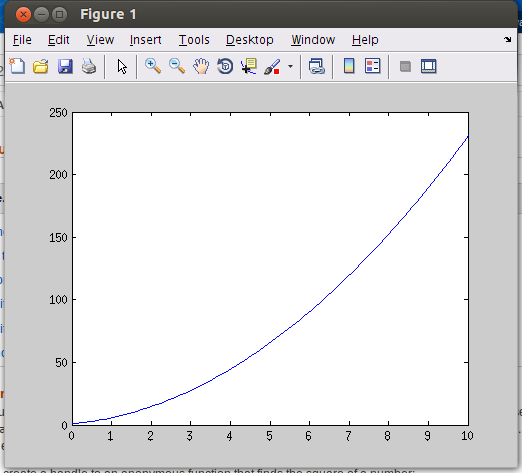
\includegraphics[width=0.4\textwidth]{./ventanafigure.png}
      \caption{\sl Ventana gr\'afica por defecto de MATLAB.}
      \label{fig:ventanagrafica}
      \end{center}
      \end{figure}
     Para crear una nueva ventana gr\'afica donde dibujar hacemos uso de la funci\'on \texttt{figure()}. Por 
     ejemplo las intrucciones
     \begin{verbatim}
      figure(1);
      ezplot(inline('x^2'));
      figure(2);
      ezplot(inline('x^2-1'));
      figure(3);
      ezplot(inline('x^2-2'));
     \end{verbatim}
     crear\'an tres ventanas gr\'aficas llamadas \texttt{Figure 1, 2 } y \texttt{3}, las cuales se abrir\'an 
     en ese orden con tres gr\'aficas muy similares.
     Si nos interesa adjuntar estos tres gr\'aficos en una misma ventana gr\'afica hacemos uso del 
     comando \texttt{hold on}, como se ilustra a continuaci\'on,
     \begin{verbatim}
     figure(4); hold on;
      ezplot(inline('x^2'));
      ezplot(inline('x^2-1'));
      ezplot(inline('x^2-2'));
     \end{verbatim}
     si finalmente no deseamos agregar m\'as gr\'aficos a esta figura ejecutamos 
     \begin{verbatim}
      hold off;
     \end{verbatim}  
     Si se desea que las gr\'aficas adjuntas cambien de colores autom\'aticamente se puede usar la instrucci\'on \texttt{hold all;} en vez de \texttt{hold on;}.
     
     Adem\'as como anotaciones podemos agregar texto en ciertos lugares de los gr\'aficos de una figura. Mientras 
     la figura en la que deseamos añadir un comentario est\'e seleccionada con el comando \texttt{figure()} ejecutamos el 
     comando \texttt{gtext()}. Si conocemos la coordenada exacta donde queremos hacer un comentario, podemos 
     utilizar la funci\'on \texttt{text()}.
     
     \subsection{Uso del comando \texttt{line()}, \texttt{label()} y opciones de estilo en gr\'aficos}
     
     A modo de ejemplo, a continuaci\'on presentamos un c\'odigo que sobrepone aproximaciones 
     en serie de Taylor de la funci\'on $y=sen(x)$ y formatea un gr\'afico con varios detalles.
     Para acceder al rutero ingrese a

     \url{http://www.udec.cl/~fmilanese/codigo4.m}
     
      l\'ealo y ejec\'utelo.
      
      \subsection{Opciones de estilo para dibujar curvas en 2D}

      Las opciones de estilo del comando \texttt{plot()} son una cadena que consiste de hasta tres 
      car\'acteres que especifican color, el estilo de l\'inea y forma de marcar los puntos de una gr\'afica.
      Estos caracteres son resumidos en la siguiente tabla
      
      \begin{center}
      \begin{tabular}{|c|c|c||}
Estilo de color & Estilo de linea & Estilo de marcador 	\\
\hline
\begin{tabular}{p{5mm}c}
 y & amarillo 	\\
 m & magenta  	\\
 r & rojo 	\\
 g & verde	\\
 b & azul	\\
 w & blanco	\\
 k & negro
\end{tabular}
&
\begin{tabular}{p{5mm}c}
 - & solida 	\\
-- & rayada  	\\
 : & punteada 	\\
-. & raya punto	\\
none & sin l\'inea \\
\end{tabular}
&
\begin{tabular}{p{5mm}c}
 + & signo de suma 	\\
 o & circulo  	\\
 * & asterisco 	\\
 x & con una equis	\\
 . & con un punto \\
$\wedge$ & tri\'angulo 	\\
 s & cuadrado 	\\
 d & diamante	\\
\end{tabular}
 \end{tabular}
 \end{center}
 
 los cuales puede ser usados como
 
 \begin{verbatim}
  plot(x,y,'r*')  %dibuja con linea roja continua y con marcadores asterisco
  plot(x,y,'b--') %dibuja con linea azul rayada
  plot(x,y,'+')   %dibuja puntos no conectados con un marcador +
 \end{verbatim}

 \section{Subgr\'aficas en una figura}

 Si qse quiere hacer un cuantos gr\'aficos dentro de una misma figura, pero 
 no sobreponerlos, se utiliza el comando \texttt{subplot()}, este comando requiere tres 
 entradas de numeros enteros \texttt{subplot(m,n,p)} y representa dividir
 la ventana gr\'afica en $m\times n$ subventanas y elegir la subventana $p-$\'esima, 
 contadas por filas, como ventana de dibujo.
 
  Por ejemplo
  \begin{verbatim}
   subplot(2,2,3)
  \end{verbatim}
  dividir\'a la ventana gr\'afica actual en cuatro subventanas y dibujar\'a lo siguiente en la ventana 
  inferior izquierda.
 
  \section{Resumen de las principales funciones para graficar 2D}

 En la siguiente tabla se encuentran las principales funciones para hacer gr\'aficas 2D.

 \begin{center}
 \begin{tabular}{|p{2cm}|c||}
 Nombre				& Descripci\'on			\\
 \hline 
  \texttt{fplot()}		& Crea un gr\'afico de una funci\'on de una variable\\
  \texttt{bar()}		& Crea un gr\'afico de barras vertical\\
  \texttt{contour()}		& Crea un gr\'afico de curvas de nivel\\
  \texttt{contourf()}		& Crea un gr\'afico de curvas de nivel llenas\\
  \texttt{polar()}		& Dibuja curvas descritas en coordenadas polares\\
  \texttt{quiver()}		& Dibuja campos vectoriales\\
 \end{tabular}
 \end{center}
 
 a continuaci\'on ejemplos de usos de estos c\'odigos.
 
 \begin{center}
  \begin{longtable}{||l|c|c||}
   Funci\'on 		& C\'odigo 		& Salida \\
   \hline

\texttt{fplot()}		
  &
\begin{minipage}{3in}
\begin{verbatim}
f='sin(x.^2+3*x)'
fplot(f,[-10,pi])
\end{verbatim}

Notar que $f$ debe estar definida en $x$.
\end{minipage}
&
\begin{minipage}{0.3\textwidth}
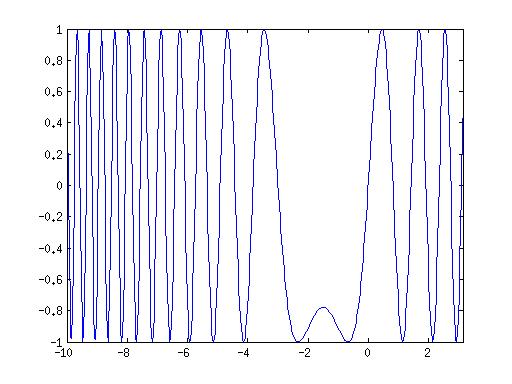
\includegraphics[width=\textwidth]{./ej1.jpg}
\end{minipage}
\\
\hline
\texttt{bar()}		
  & 
\begin{minipage}{3in}
\begin{verbatim}
t=linspace(0,2*pi,200);
r=sqrt(abs(2*sin(5*t))) ;
y=r.*sin(t);
bar(t,y);
axis([0 pi 0 inf ]);
\end{verbatim}
\end{minipage}
&
\begin{minipage}{0.3\textwidth}
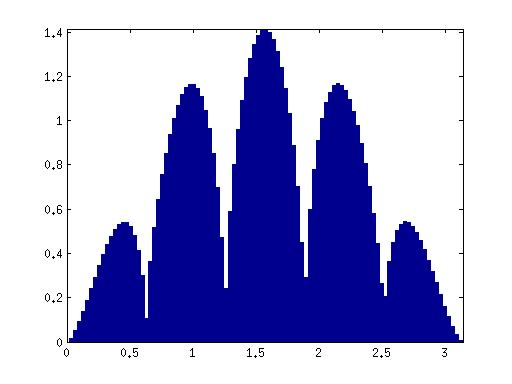
\includegraphics[width=\textwidth]{./ej2.jpg}
\end{minipage}
\\
\hline
  \texttt{contour()}		& 
\begin{minipage}{3in}
\begin{verbatim}
r =-5:.2:5;
[X,Y]=meshgrid(r,r) ;
Z=-.5*X.^2 +X.*Y+Y.^2;
cs=contour(X,Y,Z);
clabel(cs);
\end{verbatim}
\end{minipage} 
&
\begin{minipage}{0.3\textwidth}
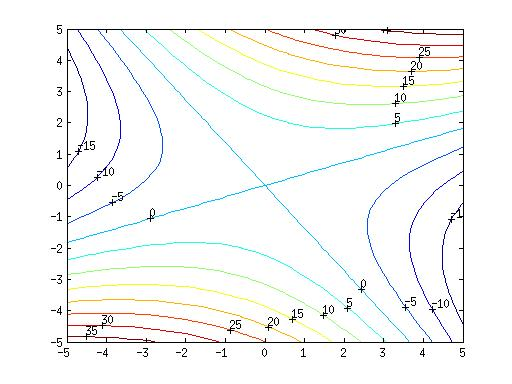
\includegraphics[width=\textwidth]{./ej3.jpg}
\end{minipage}
\\
\hline
  \texttt{polar()}		& 
\begin{minipage}{3in}
\begin{verbatim}
t=linspace(0,2*pi,200);
r=sqrt(abs(2*sin(5*t))) ;
polar(t,r);
\end{verbatim}
\end{minipage} 
&
\begin{minipage}{0.3\textwidth}
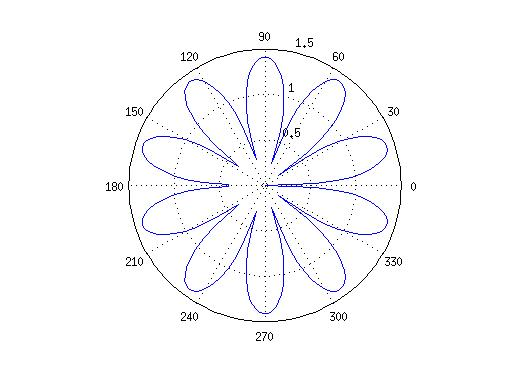
\includegraphics[width=\textwidth]{./ej4.jpg}
\end{minipage}
\\
\hline
  \texttt{quiver()}		& 
\begin{minipage}{3in}
\begin{verbatim}
r=-2:.2:2;
[X,Y]=meshgrid(r,r) ;
Z=X.^2-5*sin(X.*Y)+Y.^2;
[dx,dy]=gradient(Z,.2,.2);
quiver(X,Y,dx,dy,2);
\end{verbatim}
\end{minipage}
&
\begin{minipage}{0.3\textwidth}
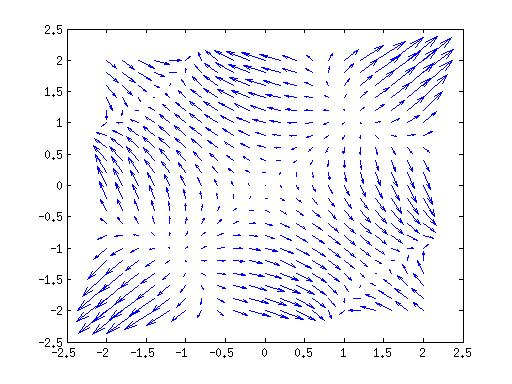
\includegraphics[width=\textwidth]{./ej5.jpg}
\end{minipage}
\\
  \end{longtable}
 \end{center}



\section{Ejercicios}
\begin{enumerate}
    \item Haga un rutero que grafique las siguientes funciones
    \begin{center}
    $f(x)=sin(x^2)^2$,  $r(x)=f(\sqrt{x})$ y $s(x)=f(r(x))$.
    \end{center}
    etiquete los ejes, titule el gr\'afico y ponga un leyenda.	
    
    \item Haga una funci\'on en MATLAB que dado $n\in N$ dibuje las primeras $n$ aproximaciones por serie de Taylor 
    de la funci\'on $cos(x)$, recuerde que la $n-$\'esima serie de taylor de una funci\'on es
    $$
    \sum_{j=0} ^ {n} \frac {f^{(j)}(0)}{j!} \, (x)^{j}.
    $$
    Puede utilizar la funci\'on de MATLAB \texttt{factorial()}.
    
    \item Haga una funci\'on MATLAB que dada una celda de funciones como arreglos haga los dibujos de estas funciones 
    en una misma ventana gr\'afica.
    
    \item Sabiendo que el comando 
    \begin{verbatim}
     datestr(now(),'hh_mm_ss_dd')
    \end{verbatim}
    retorna una cadena con la fecha actual en el formato ``hora\_minutos\_segundos\_dia'' haga una funci\'on MATLAB
    que dada una funci\'on y un t\'itulo grafique la funci\'on y le ponga como subtitulo la fecha actual. Use las funciones  
 \texttt{title()} y \texttt{subtitle()}.
    
    \item Sabiendo que el comando
    \begin{verbatim}
     print -djpeg85 -r300 matilda
    \end{verbatim}
    graba una imagen de la ventana gr\'afica actual en el archivo \texttt{matilda.jpeg} 
    ubicado en el directorio actual, haga una funci\'on MATLAB que dada una funci\'on la grafique y grabe la gr\'afica 
    con un nombre de la fecha a la que fue generada.

 \item  
 Construya una funci\'on que grafique y grabe ,en el directorio actual, la gr\'afica de una 
 funci\'on en formato \texttt{.jpeg} o \texttt{.jpg}. Utilice esta 
 funci\'on para generar las gr\'aficas de las funciones.
\begin{multicols}{2}
 \begin{itemize}
  \item[a)] $f(x)=\begin{cases}
                   x^2+2x	& \text{ si } x>1\\
                   x		& \text{ si } x\in [0,1]\\
                   -2*x		& \text{ si } x<0
                  \end{cases}$ 

  \item[b)] $g(x)=f(f(x))$
  \item[c)] $r(x)=f(f(x^2+1))$
  \item[d)] $h(x)=\begin{cases}
                   e^{x}+sin(x)	& \text{ si } x>1\\
                   x+x^2		& \text{ si } x\in [0,1]
                  \end{cases}$ 

  \item[e)] $i(x)=h(h(x))$
  \item[f)] $j(x)=h(h(cos(x)+1))$
 \end{itemize}
 \end{multicols}
 
 
 \item
Decida gr\'aficamente si la funci\'on $h(x,y)=\frac{1}{x^2+y^2-2}$ presenta alguna discontinuidad. Haga un bosquejo de esta funci\'on.
 
 
 \item Haga un rutero que construya una animaci\'on de las gr\'aficas  de la funci\'on 
 $ f(x)=cos(e^{n \,x})$ versus $x$, cuando $n\in [-1,1]$ es el par\'ametro que var\'ia en el tiempo y $x\in[-\pi,\pi]$ son los puntos del dominio de $f$.
 

\item El desarrollo en serie de Fourier de la funci\'on 
$$
f(x)=
\begin{cases}
0 & \text{, si } x\in[-\pi,0]\\
\pi-x & \text{, si } x\ in[0,\pi]
\end{cases}
$$
est\'a dado por la serie de funciones
$$
\displaystyle
f(x)=\frac{\pi}{4} + \sum_{n=1}^\infty \, \frac{1-(-1)^n}{n^2\pi} cos(nx)+ \frac{1}{n} sen(nx),
$$
haga un rutero que grafique las primeras diez sumas parciales de esta suma funciones y la funci\'on $f$ en el intervalo $[-2\pi,2\pi]$.


\item Construya un rutero llamado \texttt{graficador.m} que construya la gr\'afica en el intervalo $[-2\pi,2\pi]$ de la funci\'on 
$$
f(x)=
\begin{cases}
sin(\pi x)  & \text{ si } x\leq 0\\
\frac{1}{x}	& \text{ si } x>0\\
\end{cases},
$$
y adem\'as que grabe esta gr\'afica como \texttt{grafica.jpg}. 

\item Descargue el archivo ubicado en 
\begin{center}
\url{http://www.udec.cl/~fmilanese/MujeresEscuelasMatrices.csv}
\end{center}
usando la funci\'on \texttt{dlmread()} lea este fichero delimitado por comas y grafique los ingresos de mujeres a las escuelas de grumetes y escuela naval para la marina Chilena.

\item Descargue el archivo ubicado en 
\begin{center}
\url{http://www.udec.cl/~fmilanese/produccioncobre.csv}
\end{center}
usando la funci\'on \texttt{dlmread()} lea este fichero delimitado por comas y grafique el porcentaje de cobre del total mundial producido por a\~no en Chile.

\end{enumerate}
\end{document}  